
\documentclass[ms.tex]{subfiles}
\begin{document}

\section{Predicted SN Ia Rates}
\label{sec:predictions}

\begin{figure*}
\centering
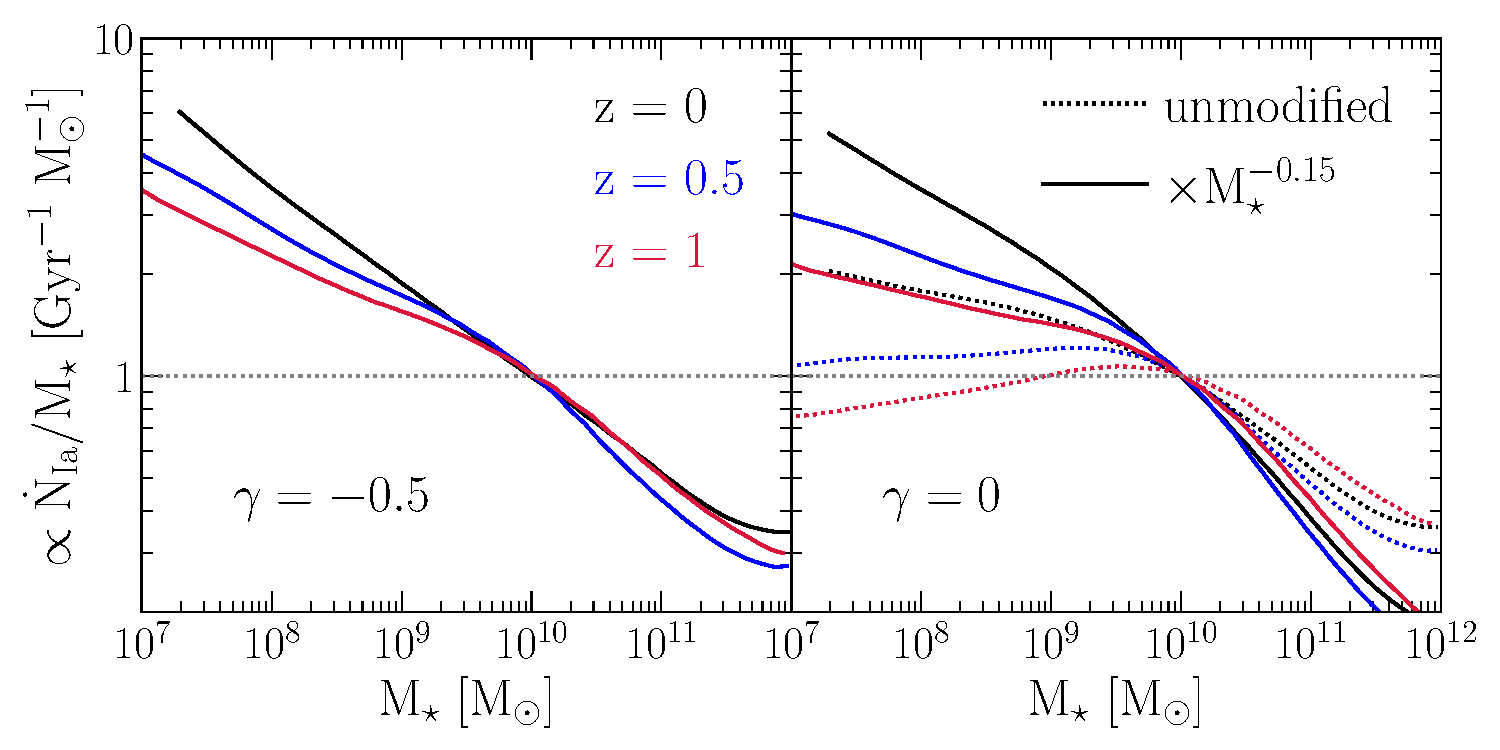
\includegraphics[scale = 0.56]{umachine_iarate_redshiftevol.pdf}
\caption{
The specific SN Ia rate as a function of stellar mass with ($\gamma = -0.5$,
left) and without ($\gamma = 0$, right) a metallicity dependence at redshifts
$z = 0$ (black),~$z = 0.5$ (blue), and~$z = 1$ (red).
Following~\citet{Brown2019} and~\citet{Gandhi2022}, we normalize all rates to
a value of 1 at~$\mstar = 10^{10}~\msun$.
In the right panel, we artificially amplify the rates by a factor of
$(M_\star / 10^{10}~\msun)^{-0.15}$ to bring the~$z = 0$ predictions into
better agreement with an~$\sim M_\star^{-0.3}$ scaling as predicted by the
$\gamma = -0.5$ case.
Stellar masses correspond to the appropriate redshift -- that is, the rates at,
e.g.,~$z = 1$ are plotted against the~$z = 1$ stellar masses and not the
present day stellar masses.
We show the unmodified rates as dotted lines (the black solid line in the left
panel and the black dotted line in the right panel are the same as the green
line and black solid line in the left panel of Fig.~\ref{fig:specia_metdep}).
}
\label{fig:specia_zdep}
\end{figure*}

We now combine the mean SFHs for galaxies of various stellar masses
from~\um~with the observed MZR in the~$10^{7.2} - 10^{12}~\msun$ range in the
framework discussed in~\S~\ref{sec:galprops}.
Given the present day stellar mass of a galaxy, we compute its SFH as a
function of lookback time by interpolating between the stellar masses and
snapshot times included in the~\um~predictions.\footnote{
	\url{https://www.peterbehroozi.com/data.html}. We interpolate linearly in
	both stellar mass and lookback time and not in the log of either
	quantity.
}
We then compute the specific SN Ia rate according to equation~\refp{eq:specia}
given the implied SFH and a~$\tau^{-1}$ DTD, artificially amplifying the rate
by a factor of~$Z^\gamma$ where the metallicity~$Z$ is computed from the
\citet{Zahid2014} MZR.
While the observationally inferred scaling with stellar mass is significantly
dependent upon the assumed SMF~\citep{Gandhi2022}, we emphasize that this
theoretical approach is independent of the SMF because we are computing the
rates using the mean SFH at a given stellar mass as opposed to from a survey
where rates within individual galaxies are not feasible to measure.
\par
We show the results of this procedure in the left panel of Fig.
\ref{fig:specia_metdep} for~$\gamma = 0$,~$-0.2$,~$-0.5$,~$-1$, and~$-2$ in
comparison to the~$\dot{N}_\text{Ia} / M_\star \sim M_\star^{-0.5}$ and
$\dot{N}_\text{Ia} / M_\star \sim M_\star^{-0.3}$ scalings derived by
\citet{Brown2019} and~\citet{Gandhi2022}, respectively.
The metallicity dependence has a significant impact only below
$\mstar \approx 3\times10^9~\msun$, a result which arises due to the shape of
the MZR; this is the mass above which the MZR flattens considerably.
Assuming no metallicity dependence (i.e.~$\gamma = 0$), these calculations
suggest that the variations in SFHs between~$\sim10^{7.2}$ and
$\sim10^{10}~\msun$ can account for only a factor of~$\sim$2 increase in the
specific SN Ia rate.
Within the observational and theoretical uncertainties, the~$\gamma = -0.5$
case is generally consistent with a mass dependence of~$M_\star^{-0.3}$, while
the steeper dependence of~$M_\star^{-0.5}$ would require a stronger scaling of
roughly~$\gamma \approx -1.5$.
\citet{Gandhi2022} advocate for a~$\gamma \approx -0.5$ scaling, additionally
demonstrating that incorporating this metallicity dependence into the
FIRE-2\footnote{
	Feedback In Realistic Environments.
	\url{https://fire.northwestern.edu/}
} cosmological zoom-in simulations~\citep{Hopkins2018} leads to better
agreement with the stellar masses and iron abundances measured by
\citet{Gallazzi2005} and~\citet{Kirby2013}.
\par
In the right panel of Fig.~\ref{fig:specia_metdep}, we compare the same
scalings to the close binary fractions in APOGEE measured by~\citet{Moe2019}.
We mark the position of~$Z \approx 10^{-0.6} Z_\odot$, the characteristic
abundance of an~$\mstar = 10^{7.2}~\msun$ galaxy according to
\citet{Zahid2014}.
Within the range of metallicities spanned by the stellar masses we explore here,
the close binary fraction is remarkably consistent with a~$\gamma = -0.5$
scaling with metallicity.
If the~$\sim M_\star^{-0.3}$ scaling found by~\citet{Gandhi2022} is accurate,
then this result suggests that the increase of the specific SN Ia rate with
decreasing stellar mass can be explained entirely by dwarf galaxies having more
extended SFHs and a higher close binary fraction due to their lower abundances.
If one instead takes~$Z \approx 0.1Z_\odot$ for a~$\sim10^{7.2}~\msun$ galaxy
as suggest by~\citet{Andrews2013}, then there is a slight tension between a
$\gamma = -0.5$ scaling and the close binary fraction measured by
\citet{Moe2019}.
If both the~\citet{Andrews2013} MZR and the~$\gamma = -0.5$ scalings are
accurate, then it would be reasonable to suggest that the additional increase
in the SN Ia rates not supplied by the increased binary fraction arise due to
more massive WDs forming at low~$Z$ -- the scenario postulated by
\citet{Kistler2013}.
Nonetheless, the scaling of the close binary fraction with metallicity can
explain the majority of the effect in this case anyway.
If instead the~$\sim M_\star^{-0.5}$ found by~\citet{Brown2019} is accurate,
then the required~$\gamma \approx -1.5$ scaling cannot be explained by the
close binary fraction alone as it would reach unphysical values ($>1$) within
the range of observed metallicities.
Such scalings are disfavored by~\citet{Gandhi2022} because they fail to
reproduce the well-known correlations between stellar [Mg/Fe] and [Fe/H]
abundances as observed in M31 satellites by~\citep*{Vargas2014} but are still
within the range of theoretical possibilities because only a small fraction of
WDs actually explode ($\sim4$\% if the progenitors are~$\sim3 - 8~\msun$
stars;~\citealp{Maoz2012b}).
In the next section, we discuss potential observational diagnostics of
a~$Z^{-0.5}$ metallicity dependence or lack thereof.

\end{document}
